                                                                            % This document is under construction

\documentclass{article}
\usepackage[utf8]{inputenc}
\usepackage{hyperref}
\usepackage{graphicx}
\usepackage{multirow}
\usepackage{mhchem}
\usepackage{gensymb}
\usepackage{mathtools}
\usepackage{float}
%\usepackage{xfrac}

\begin{document}

\title{Solution to the exercises of the book ``Introduction to Rocket Science and Engineering''}
\author{Arturo Gonzalez\\
	\texttt{\href{mailto:arturo.gonzalez@argonur.com}{arturo.gonzalez@argonur.com}}}
\date{\today}
\maketitle

\begin{abstract}
This document contains the solution to the exercises of each chapter of the book ``Introduction to Rocket Science and Engineering'' by Travis S. Taylor. Solving the exercises is a project proposed in the blog \url{https://www.argonur.com}.\\

To visit the website of the project: \\
\url{https://argonur.com/solucion-introduction-to-rocket-science-and-engineering/}.\\

If you find errors in the document, want to participate solving the exercises of the book, etc., please send an email to \href{mailto:arturo.gonzalez@argonur.com}{arturo.gonzalez@argonur.com}
\end{abstract}

\cleardoublepage
%%%%%%%%%%%%%%%%%%%%%%%%%%%%%
%	Chapter 1				%
%%%%%%%%%%%%%%%%%%%%%%%%%%%%%

\section{Exercises of Chapter 1}

\begin{enumerate}
	\item {\bf Discuss the relevance of the \textit{aelopile} to rocket science and why it was considered the first demonstration of the principle of rocketry.}\\

The aeolipile consists of a vessel, usually a "simple" solid of revolution, such as a sphere or a cylinder, arranged to rotate on its axis, having oppositely bent or curved nozzles projecting from it (tipjets). When the vessel is pressurised with steam, steam is expelled through the nozzles, which generates thrust due to the rocket principle as a consequence of the 2nd and 3rd of Newton's laws of motion. When the nozzles, pointing in different directions, produce forces along different lines of action perpendicular to the axis of the bearings, the thrusts combine to result in a rotational moment (mechanical couple), or torque, causing the vessel to spin about its axis. \cite{aeolipile}

	\item {\bf What are the main components of the gunpowder?}\\
	
Gunpowder, also known as black powder, is the earliest known chemical explosive. It is a mixture of sulfur, charcoal, and potassium nitrate (saltpeter). The sulfur and charcoal act as fuels, and the saltpeter is an oxidizer. Because of its burning properties and the amount of heat and gas volume that it generates, gunpowder has been widely used as a propellant in firearms, as a pyrotechnic composition in fireworks and as a blasting powder in quarrying, mining, and road building. \cite{gunpowder}
	
	\item {\bf What was \textit{Principia} and why is it relevant to rocket science?}\\

\textit{\textbf{Philosophiæ Naturalis Principia Mathematica}} (Latin for Mathematical Principles of Natural Philosophy), often referred to as simply the \textit{Principia}, is a work in three books by Isaac Newton, in Latin, first published 5 July 1687. After annotating and correcting his personal copy of the first edition, Newton published two further editions, in 1713 and 1726. The \textit{Principia} states Newton's laws of motion, forming the foundation of classical mechanics; Newton's law of universal gravitation; and a derivation of Kepler's laws of planetary motion (which Kepler first obtained empirically). The \textit{Principia} is one of the most important works in the history of science. \cite{principia}

It was through these laws of motion that other scientists and engineers could understand the whys and hows of rockets and rocket science.

Standing on Newton’s foundations and with the development of calculus by he and Gottfried Leibniz (independently), the 1700s brought forth even greater understanding of rocketry. \cite{book}
	
	\item {\bf Why were William Hale’s rockets “better” than William Congreve’s?}\\

In 1844, the Congreve rockets were replaced by ones designed by the English inventor, William Hale. Hale had been developing the “stickless rocket” for nearly two decades. The Congreve rockets used the stick concept for stabilization much in the same way seen on modern bottle rockets. Hale used three fins mounted on the rocket for stabilization. The rocket also was known to spin when launched and was often referred to as the “rotary rocket.” This was actually the development of spin stabilization, which is used by many modern rockets today. \cite{book}

	\item {\bf Compare and contrast the contributions to the development of rocketry by Konstantin Tsiolkovsky and Robert Goddard. Which one could be considered the “father of rocket science” and which one the “father of rocket engineering”?}\\
	
{\bf Konstantin Tsiolkovsky}\\
Konstantin Eduardovich Tsiolkovsky (17 September 1857  – 19 September 1935) was a Russian and Soviet rocket scientist and pioneer of the astronautic theory.

Tsiolkovsky stated that he developed the theory of rocketry only as a supplement to philosophical research on the subject. He wrote more than 400 works including approximately 90 published pieces on space travel and related subjects. Among his works are designs for rockets with steering thrusters, multistage boosters, space stations, airlocks for exiting a spaceship into the vacuum of space, and closed-cycle biological systems to provide food and oxygen for space colonies. \cite{konstantin}
\\

{\bf Robert H. Goddard}\\
Robert Hutchings Goddard (October 5, 1882 – August 10, 1945) was an American engineer, professor, physicist, and inventor who is credited with creating and building the world's first liquid-fueled rocket. Goddard successfully launched his model on March 16, 1926 ushering in an era of space flight and innovation. He and his team launched 34 rockets between 1926 and 1941, achieving altitudes as high as 2.6 km (1.6 mi) and speeds as fast as 885 km/h (550 mph).

Goddard's work as both theorist and engineer anticipated many of the developments that were to make spaceflight possible. He has been called the man who ushered in the Space Age. Two of Goddard's 214 patented inventions — a multi-stage rocket (1914), and a liquid-fuel rocket (1914) — were important milestones toward spaceflight. His 1919 monograph A Method of Reaching Extreme Altitudes is considered one of the classic texts of 20th-century rocket science. Goddard successfully applied three-axis control, gyroscopes and steerable thrust to rockets, to effectively control their flight. \cite{goddard}

{\bf Konstantin Tsiolkovsky} can be considered as the father of rocket science for all of his theoretical work in the field. He derived formulas for aeronautics and conceived ideas that have been used in rockets. He never built a rocket.

{\bf Robert H. Goddard} can be considered the father of rocket engineering for all of his experimental work with rockets. He not only recognized the potential of rockets for atmospheric research, ballistic missiles and space travel but was the first to scientifically study, design and construct the rockets needed to implement those ideas.

	\item {\bf Who was known as the Chief Designer and why?}\\
	
{\bf Sergei Pavlovich Korolev} worked as the lead Soviet rocket engineer and spacecraft designer during the Space Race between the United States and the Soviet Union in the 1950s and 1960s. He is considered by many as the father of practical astronautics.

Although Korolev trained as an aircraft designer, his greatest strengths proved to be in design integration, organization and strategic planning. Arrested for alleged mismanagement of funds (he spent the money on unsuccessful experiments with rocket devices), he was imprisoned in 1938 for almost six years, including some months in a Kolyma labour camp. Following his release he became a recognized rocket designer and a key figure in the development of the Soviet Intercontinental ballistic missile program. He was then appointed to lead the Soviet space program and made a Member of Soviet Academy of Sciences, overseeing the early successes of the Sputnik and Vostok projects including the first human Earth orbit mission by Yuri Alexeevich Gagarin on 12 April 1961. Korolev's unexpected death in 1966 interrupted implementation of his plans for a Soviet manned Moon landing before the United States 1969 mission.

Before his death he was officially identified only as Glavny Konstruktor, or the Chief Designer, to protect him from possible cold war assassination attempts by the United States. Only following his death in 1966 has he received appropriate public recognition as the driving force behind Soviet accomplishments in space exploration during and following the International Geophysical Year. \cite{korolev}
	
	\item {\bf Who was the Chief Designer’s counterpart in the American space program?}\\
	
{\bf Wernher Magnus Maximilian Freiherr von Braun} (March 23, 1912 – June 16, 1977) was a German, later American, aerospace engineer and space architect credited with inventing the V-2 rocket for Nazi Germany and the Saturn V for the United States. He was one of the leading figures in the development of rocket technology in Nazi Germany, where he was a member of the Nazi Party and the SS.

Following World War II, he was secretly moved to the United States, along with about 1,500 other scientists, engineers, and technicians, as part of Operation Paperclip, where he developed the rockets that launched the United States' first space satellite Explorer 1, and the Apollo program manned lunar landings.

In his twenties and early thirties, von Braun worked in Germany's rocket development program, where he helped design and develop the V-2 rocket at Peenemünde during World War II. Following the war, von Braun worked for the United States Army on an intermediate-range ballistic missile (IRBM) program before his group was assimilated into NASA. Under NASA, he served as director of the newly formed Marshall Space Flight Center and as the chief architect of the Saturn V launch vehicle, the superbooster that propelled the Apollo spacecraft to the Moon. In 1975, he received the National Medal of Science. He continued insisting on the human mission to Mars throughout his life. \cite{vonbraun}
	
	\item {\bf What is the oldest spacecraft still in orbit?}\\
	
Vanguard 1 (ID: 1958-Beta 2) was the fourth artificial Earth orbital satellite launched (after Sputnik 1, Sputnik 2, and Explorer 1). It was the first satellite to be solar powered. Although communication with it was lost in 1964, it remains the oldest manmade satellite still in orbit. It was designed to test the launch capabilities of a three-stage launch vehicle as a part of Project Vanguard, and the effects of the environment on a satellite and its systems in Earth orbit. It also was used to obtain geodetic measurements through orbit analysis. Vanguard 1 was described by then-Soviet Premier Nikita Khrushchev as, "The grapefruit satellite." \cite{vanguard1}
	
	\item {{\bf What is UDMH? What is it used for? What is NTO?}}\\

{\bf UDMH}\\
Unsymmetrical dimethylhydrazine (UDMH; 1,1-dimethylhydrazine) is a chemical compound with the formula \ce{H2NN(CH3)2}. It is a colourless liquid, with a sharp, fishy, ammoniacal smell typical for organic amines. Samples turn yellowish on exposure to air and absorb oxygen and carbon dioxide. It mixes completely with water, ethanol, and kerosene. In concentration between 2.5\% and 95\% in air, its vapors are flammable. It is not sensitive to shock.

UDMH is often used in hypergolic rocket fuels as a bipropellant in combination with the oxidizer nitrogen tetroxide and less frequently with IRFNA (red fuming nitric acid) or liquid oxygen. UDMH is a derivative of hydrazine and is sometimes referred to as a hydrazine.

UDMH is often used in hypergolic rocket fuels as a bipropellant in combination with the oxidizer nitrogen tetroxide and less frequently with IRFNA (red fuming nitric acid) or liquid oxygen. UDMH is a derivative of hydrazine and is sometimes referred to as a hydrazine. \cite{udmh}

{\bf NTO}\\
Dinitrogen tetroxide, commonly referred to as nitrogen tetroxide, is the chemical compound \ce{N2O4}. It is a useful reagent in chemical synthesis. It forms an equilibrium mixture with nitrogen dioxide.

Dinitrogen tetroxide is a powerful oxidizer that is hypergolic (spontaneously reacts) upon contact with various forms of hydrazine, which makes the pair a popular bipropellant for rockets.

Nitrogen tetroxide is used as an oxidizer in one of the more important rocket propellants because it can be stored as a liquid at room temperature. In early 1944 research on the usability of dinitrogen tetroxide as an oxidizing agent for rocket fuel was conducted by German scientists, although the Nazis only used it to a very limited extent as an additive for S-Stoff (fuming nitric acid). It became the storable oxidizer of choice for many rockets in both the United States and USSR by the late 1950s. It is a hypergolic propellant in combination with a hydrazine-based rocket fuel. One of the earliest uses of this combination was on the Titan family of rockets used originally as ICBMs and then as launch vehicles for many spacecraft. Used on the U.S. Gemini and Apollo spacecraft and also on the Space Shuttle, it continues to be used as stationkeeping propellant on most geo-stationary satellites, and many deep-space probes. It now seems likely that NASA will continue to use this oxidizer in the next-generation 'crew-vehicles' which will replace the shuttle. It is also the primary oxidizer for Russia's Proton rocket.

When used as a propellant, dinitrogen tetroxide is usually referred to simply as 'Nitrogen Tetroxide' and the abbreviation 'NTO' is extensively used. Additionally, NTO is often used with the addition of a small percentage of nitric oxide, which inhibits stress-corrosion cracking of titanium alloys, and in this form, propellant-grade NTO is referred to as "Mixed Oxides of Nitrogen" or "MON". \cite{nto}
	
	\item {\bf Draw a simple liquid fuel rocket and label all the major subcomponents.}\\

[ Drawing of a liquid fuel rocket with labels of major components to be added ]\\

The major components are:
\begin{itemize}

	\item {\bf Structure}: Provides support structure for all the components, protects the inner workings of the vehicle, contains fairings and interfaces for subsystems and stages, and houses and/or supports moving components.
	\item {\bf Propulsion}: Contains the fuel, oxidizer, flow systems, combustion chamber, nozzles, and other aspects needed for propelling the vehicle.
	\item {\bf Power}: This subsystem contains power storage, conditions that power for use, and distributes it accordingly.
	\item {\bf Guidance, Navigation, and Control (GN\&C)}: Contains attitude control system (ACS), reaction control systems (RCS); these might include thrust vector controls (TVC) and control surfaces, such as fins or wings; navigational sensors, such as inertial navigation units (INUs) and star trackers; and has computer subsystems to run GN\&C functions.
	\item {\bf Payload}: This is the reason for the rocket and contains the science instruments, cargo, or crew.
	\item {\bf Command and Data Handling (C\&DH)}: Has command computers, data processors, data storage systems, and the data distribution protocols and infrastructure.
	\item {\bf Communications (Comm)}: Contains radios, low and high gain antennas, and telemetry systems.
	\item {\bf Reentry Systems}: These are for rockets that must safely return a payload to Earth and contain braking systems, such as the orbital maneuvering system (OMS) thrusters on the Space Shuttle, and reentry thermal protection, such as the shuttle tiles or the ceramic shields on the Apollo capsules.
	\item {\bf Emergency Systems}: These systems are for use in fault condition situations and include sensors for leak, fire, and damage detection, backup systems, and abort systems like the abort rockets on the Ares I, as discussed previously.
	\item {\bf Landing Systems}: For return vehicles there must be some means of landing the payload safely on Earth, which could include parachutes, wings, airbags, or even rockets. \cite{book}


\end{itemize}


\end{enumerate}

\cleardoublepage
%%%%%%%%%%%%%%%%%%%%%%%%%%%%%
%	Chapter 2	   		    %
%%%%%%%%%%%%%%%%%%%%%%%%%%%%%

\graphicspath{{Chapter2/}}
\section{Exercises of Chapter 2}

\begin{enumerate}

	\item {\bf Discuss the dichotomy of rocket science in the modern era.}\\
	
The first dichotomy starts after WWI, with the Treaty of Versailles that prohibited Germany to develop long-range artillery and the NAZI Germany developed the V2 (\textit{Vergeltungswaffe 2}), that was a missile capable of reaching an objective 300 km away from the launch place. The ''success'' of this lethal weapon, led the governments of the Soviet Union and USA to start developing their own missiles.

The second dichotomy happens when the Soviets where the firsts to place a satellite in orbit (Sputnik), and with this, the space era started. The objective of building rockets was not anymore only military, but it was also scientific and even commercial. 

	\item {\bf In your own words give a definition for a rocket mission.}\\
	
A mission is the objective that the government of a country or a private organization has for which a rocket is needed to be accomplished. Examples are; putting a satellite in GEO, sending a robot to Mars to make experiments, sending a missile with an atomic bomb to an asteroid that is going to impact our beautiful home planet.
	
	\item {\bf What is a payload?}\\
	
The payload is the equipment that solves the problem represented by the mission. In other words, the payload is how the mission is intended to be accomplished.

For the mission \lq\lq{}putting a satellite in GEO\rq\rq{}, the payload is the satellite.\\
For the mission \lq\lq{}sending a robot to Mars to make experiments\rq\rq{}, the payload is the robot.\\
For the mission \lq\lq{}sending a missile with an atomic bomb to an asteroid that is going to impact our beautiful home planet\rq\rq{}, the payload is the bomb.

The payload is the all hardware above the launch vehicle, except the protective fairing, which is also part of the launch vehicle. 
	
	\item {\bf What is the so-called “SMAD”?}\\
	
SMAD stands for \textit{Space Mission Analysis and Preparation}, and it is the name of book, that according to \cite{book}, is the standard text book for space mission preparation.
	
	\item {\bf Give the four basic assumptions required for understanding the basics of projectile motion.}\\
	
\begin{enumerate}
1. Acceleration due to gravity is constant\\
2. No air resistance\\
3. Earth is flat\\
4. Earth’s rotation has no impact on the motion of the projectile.
\end{enumerate}
	
	\item {\bf Define MECO.}\\
	
MECO stands for main engine cutoff, and it happens when the main engine is turned off, it can be because all the propellant has been used, or also in a multistage rocket it can be that the first stage that contains the main engine still has propellant which is going to be used for the landing of the first stage.
	
	\item {\bf Equation 2.9 gives the parabolic flight path of a rocket trajectory as height, \textit{y}, as a function of range, \textit{x}, or \textit{y(x)}. Use the quadratic equation to solve for \textit{x} as a function of \textit{y} to give a range equation as a function of height.}\\

\begin{equation} \label{eq:x_of_y}
	x(y-y_{bo})  = \frac{v_{bo}^2 \cos\theta}{g}(\sin\theta \pm \sqrt{\sin^2\theta-\frac{2g(y-y_{bo})}{v_{bo}^2}})+ x_{bo} 
\end{equation}

Figure \ref{fig:exercise7} shows \textit{x(y)}.
	
\begin{figure}[H]
	\centering
	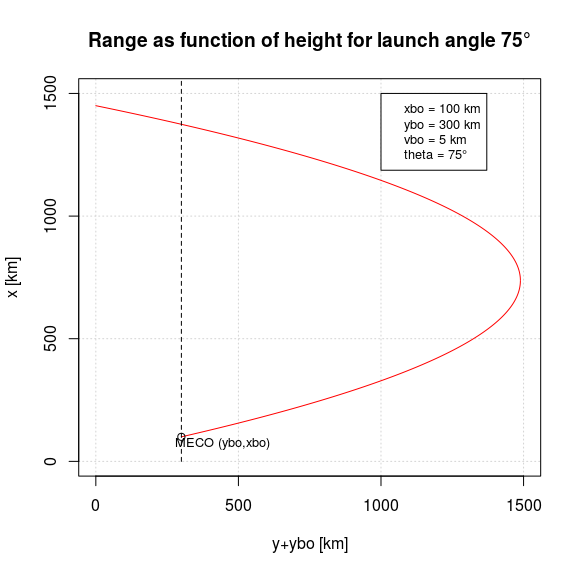
\includegraphics[width=0.7\textwidth]{exercise7.png}
	\caption{Range as a function of height \textit{x(y)}.}
	\label{fig:exercise7}
\end{figure}	
	
	\item {\bf A rocket is launched with a burnout velocity of 75 m/sec, burnout altitude of 300 m, and a burnout range of 100 m. Assuming a flight path angle of 75\degree, calculate the final range of the rocket when it impacts the ground.}\\

Substituting values into eq. 2.14 from the book. \\

\begin{equation}
	x_{max}  = x_{bo} + (v_{bo}\cos\theta)\left[ \frac{v_{bo}\sin\theta+\sqrt{v_{bo}^2\sin^2\theta+2gy_{bo}}}{g}\right]
\end{equation}

\begin{equation}
	x_{max}  =  100 + (75\cos75\degree)\left[ \frac{75\sin75\degree+\sqrt{75^2\sin^2(75\degree)+2(9.81)(300)}}{9.81}\right] = 452.1426 [m] 
\end{equation}

This value can also be observed in figure \ref{fig:exercises_8_9_10}.
	
	\item {\bf Calculate the maximum altitude reached by the rocket in Exercise 8.}\\
	
Substituting values into eq. 2.11 from the book. \\

\begin{equation}
	y_{max}  =  y_{bo} + \frac{v_{bo}^2 \sin^2\theta}{2g}
\end{equation}

\begin{equation}
	y_{max}  =  300 + \frac{75^2 \sin^2 75\degree}{2(9.81)} = 567.49 [m]
\end{equation}	

This value can also be observed in figure \ref{fig:exercises_8_9_10}.

	\item {\bf Redo Exercise 8 to determine the range at MECO altitude. What is the range at MECO if the initial flight path angle is 15\degree ?}\\
	
As explained in the book, the range at MECO for two angles whose addition equals 90\degree (75\degree + 15\degree = 90 \degree), the range at MECO is the same. Substituting values into equation \ref{eq:x_of_y} the range at MECO for 75\degree and 15\degree can be obtained.

\begin{equation}
	x(y_{MECO}-300)  = \frac{75^2 \cos15\degree}{9.81}(\sin15\degree + \sqrt{\sin^2 15\degree -\frac{2(9.81)(300-300)}{75^2}})+ 100 = 386.697 [m]
\end{equation}	
	
\begin{figure}[H]
	\centering
	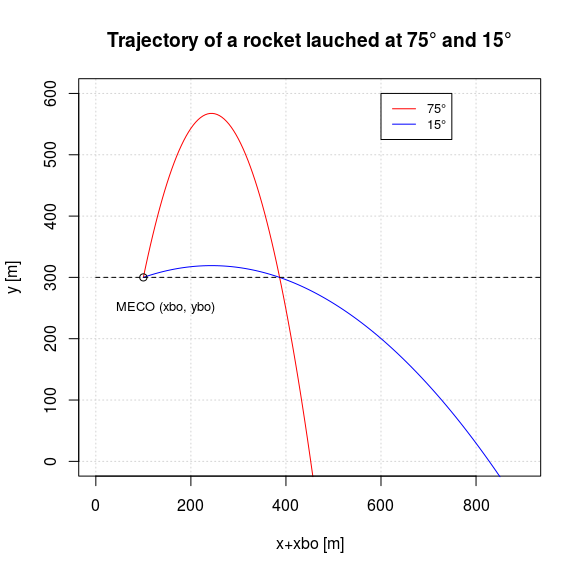
\includegraphics[width=0.7\textwidth]{exercises_8_9_10.png}
	\caption{Trajectory of rocket launched at 75\degree and 15\degree .}
	\label{fig:exercises_8_9_10}
\end{figure}

	\item {\bf What is the force due to gravitational attraction between the Earth and the Moon? Assume the Moon is 400,00 km from Earth and the mass of the Earth is $5.99 x 10^{24}$ kg, and the mass of the Moon is $7.36 x 10^{22}$ kg.} 	

	\item {\bf  A satellite is in a circular orbit at 100 km above the Earth. What is the orbital velocity of the satellite? How long does it take for the satellite to make one complete orbit around the Earth?} \\
	
	\item {\bf What is the semilatus rectum?} \\
	
	\item {\bf  Give the equation for a conic section.} \\
	
	\item {\bf  A spacecraft is traveling in an orbit with periapsis at 100 km and apoapsis at 1000 km. What is the eccentricity of the orbit? This orbit is what type of conic section?} \\
	
	\item {\bf Calculate the semilatus rectum of the spacecraft orbit in Exercise 15.} \\
	
	\item {\bf What is the period of the orbit described in Exercise 15?} \\
	
	\item {\bf What is the velocity of the spacecraft in Exercise 15?} \\
	
	\item {\bf Calculate the  $\Delta v$ needed to circularize an elliptical orbit with an apoapsis at 500 km above the Earth and a periapsis at 325 km above the Earth. (Hint: see Example 2.3.)} \\
	
	\item {\bf Calculate the $\Delta v$ burns needed to conduct a Hohmann transfer from a 300 km circular orbit around Earth to a 35,000 km circular orbit around Earth.} \\	
	
	\item {\bf Calculate the transfer time for the Hohmann transfer given in Exercise 20.} \\	

	\item {\bf A Space Shuttle is in a 325 km circular orbit in a 28\degree inclination. How much $\Delta v$ is needed to move the Shuttle to a 51\degree inclination?} \\	

	\item {\bf What is $C_3$} \\	

	\item {\bf A Mars probe leaves Earth’s sphere of influence with a $C_3$ of 16 $km^2/sec^2$. How much $\Delta v$ is required for the probe to enter a Mars orbit
with periapsis at 100 km and apoapsis at 1,000 km?} \\	

	\item {\bf In order to go from Equation 2.87 to Equation 2.88 (as well as Equation 2.89 and Equation 2.90) some algebra was needed. Do the algebra calculation showing all the steps.} \\	

	\item {\bf A ballistic missile has a powered flight range angle of 4\degree and a reentry range angle of 5\degree. If the missile has a total ground range of 8,000 km, what is its free-flight range angle? (Hint: Assume the 8,000 km range is the distance the missile travels around the circumference of the Earth. The radius of the Earth is 6,370 km.)} \\	
	
\end{enumerate}




























\cleardoublepage
%%%%%%%%%%%%%%%%%%%%%%%%%%%%%
%	References				%
%%%%%%%%%%%%%%%%%%%%%%%%%%%%%

\begin{thebibliography}{99}

\bibitem{book}
	Travis S. Taylor,
	\emph{Introduction to Rocket Science and Engineering}.
	CRC Press,
	2009.
	
\bibitem{aeolipile}
	Aeolipile\\
	Wikipedia, the free encyclopedia\\
	April 2017\\
	\url{https://en.wikipedia.org/wiki/Aeolipile}
	
\bibitem{gunpowder}
	Gunpowder\\
	Wikipedia, the free encyclopedia\\
	April 2017\\
	\url{https://en.wikipedia.org/wiki/Gunpowder}

\bibitem{principia}
	\textit{Philosophiæ Naturalis Principia Mathematica}\\
	Wikipedia, the free encyclopedia\\
	April 2017\\
	\url{https://en.wikipedia.org/wiki/Philosophiae_Naturalis_Principia_Mathematica}
	
\bibitem{konstantin}
	Konstantin Tsiolkovsky\\
	Wikipedia, the free encyclopedia\\
	April 2017\\
	\url{https://en.wikipedia.org/wiki/Konstantin_Tsiolkovsky}
	
\bibitem{goddard}
	Robert H. Goddard\\
	Wikipedia, the free encyclopedia\\
	April 2017\\
	\url{https://en.wikipedia.org/wiki/Robert_H._Goddard}	
	
\bibitem{korolev}	
	Sergei Korolev\\
	Wikipedia, the free encyclopedia\\
	April 2017\\
	\url{https://en.wikipedia.org/wiki/Sergei_Korolev}	

\bibitem{vonbraun}	
	Wernher von Braun\\
	Wikipedia, the free encyclopedia\\
	April 2017\\
	\url{https://en.wikipedia.org/wiki/Wernher_von_Braun}

\bibitem{vanguard1}
	Vanguard 1\\
	Wikipedia, the free encyclopedia\\
	April 2017\\
	\url{https://en.wikipedia.org/wiki/Vanguard_1}
	
\bibitem{udmh}
	Unsymmetrical dimethylhydrazine\\
	Wikipedia, the free encyclopedia\\
	April 2017\\
	\url{https://en.wikipedia.org/wiki/Unsymmetrical_dimethylhydrazine}
	
\bibitem{nto}
	Dinitrogen tetroxide\\
	Wikipedia, the free encyclopedia\\
	April 2017\\
	\url{https://en.wikipedia.org/wiki/Dinitrogen_tetroxide}



\end{thebibliography}

\end{document}
\grid
\grid
\grid
\grid
